\section{Related Work} \label{sec:related_work}
\textbf{Representation learning for visual model-based reinforcement learning:}
Prior works have proposed learning video prediction models~\citep{wichers2018hierarchical,denton2017unsupervised,lee2018stochastic,finn2016unsupervised} to improve exploration~\citep{oh2015action} and planning~\citep{finn2017deep} in RL.
However, such works and others that represent the scene with a single representation vector~\citep{hafner2018learning,zhang2018solar,mnih-dqn-2015,oh2016control} may be susceptible to the binding problem~\citep{greff2015binding,rosenblatt1961principles} and must rely on data to learn that the same object in two different contexts can be modeled similarly.
But processing a disentangled latent state with a single function~\citep{whitney2016understanding,chen2016infogan,kulkarni2015deep,kulkarni2019unsupervised,goel2018unsupervised} or processing each disentangled factor in a permutation-sensitive manner~\citep{lee2018stochastic,xu2019unsupervised,kulkarni2019unsupervised} (1) assumes a fixed number of entities that cannot be dynamically adjusted for generalizing to more objects than in training and (2) has no constraints to enforce that multiple instances of the same entity in the scene be modeled in the same way.
For generalization, often the particular arrangement of objects in a scene does not matter so much as what is constant across scenes -- properties of individual objects and inter-object relationships -- which the inductive biases of these prior works do not capture.
The entity abstraction in OP3 enforces symmetric processing of entity representations, thereby overcoming the limitations of these prior works.

\textbf{Unsupervised grounding of abstract entity variables in concrete objects:}
Prior works that model entities and their interactions often pre-specify the identity of the entities~\citep{chang2016compositional,battaglia2016interaction,hamrick2017metacontrol,janner2018representation,narasimhan2018grounding,bapst2019structured,ajay2019combining}, provide additional supervision~\citep{girshick2014rich,he2017mask,wang2018deep,yang2018visual}, or provide additional specification such as segmentations~\citep{janner2018reasoning}, crops~\citep{fragkiadaki2015learning}, or a simulator~\citep{wu2017learning,kansky2017schema}.
Those that do not assume such additional information often factorize the entire scene into pixel-level entities~\citep{santoro2017simple,zambaldi2018deep,du2019task}, which do not model objects as coherent wholes.
None of these works solve the problem of grounding the entities in raw observation, which is crucial for autonomous learning and interaction.
OP3 builds upon recently proposed ideas in grounding entity representations via inference on a symmetrically factorized generative model of static~\citep{greff2015binding,greff2017neural,greff2019iodine} and dynamic~\citep{van2018relational} scenes, whose advantage over other methods for grounding~\citep{zhu2019object,eslami2016attend,burgess2019monet,kosiorek2018sequential,watters2019cobra} is the ability to refine the grounding with new information.
In contrast to other methods for binding in neural networks~\citep{levy2008vector,kanerva2009hyperdimensional,smolensky1990tensor,vaswani2017attention}, formulating inference as a mechanism for variable binding allows us to model uncertainty in the values of the variables.

\begin{figure}[!t]
    \centering
    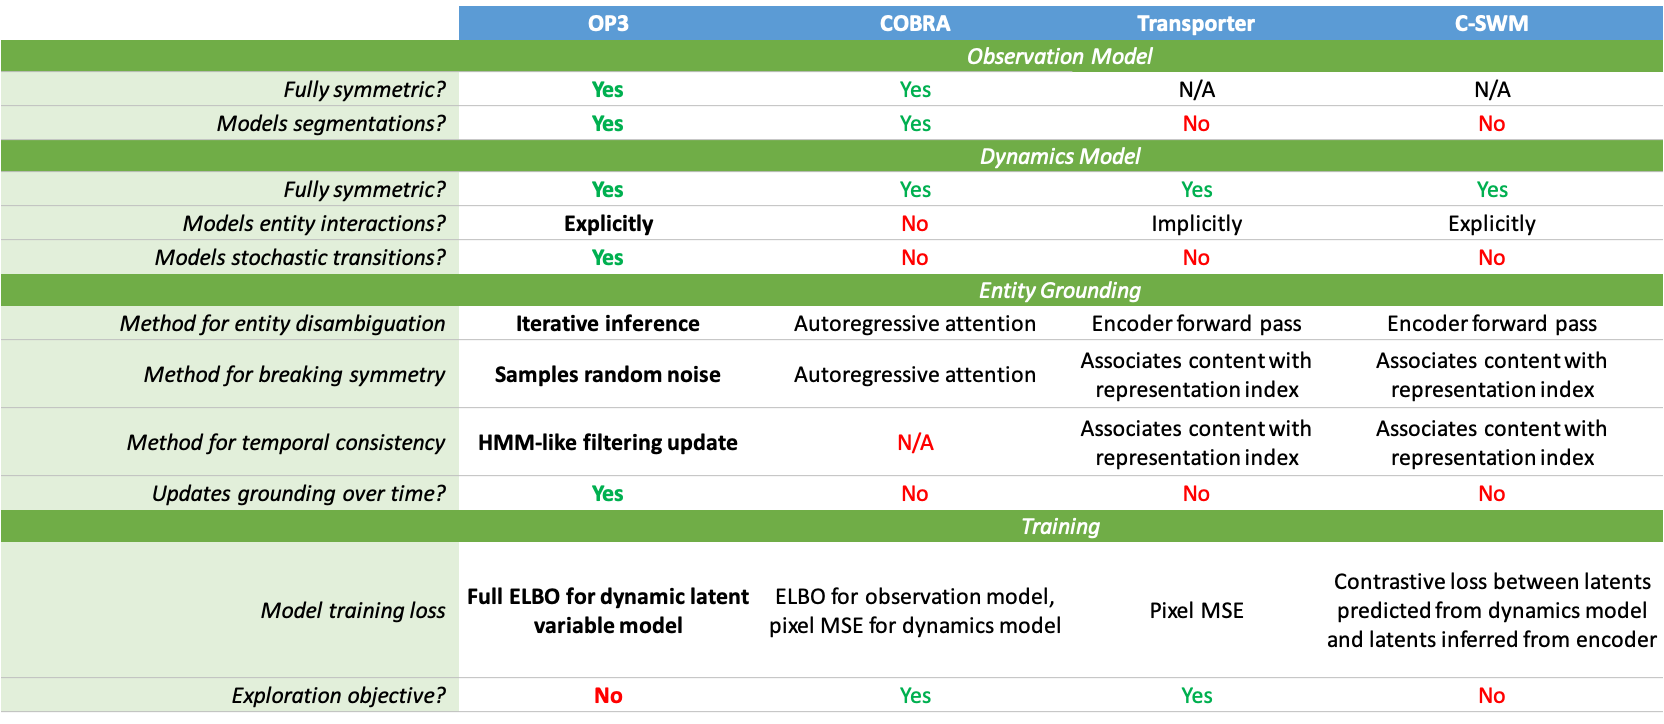
\includegraphics[width=\textwidth]{figs/method/comparison_table.png}
    \caption{\small{
    \textbf{Comparison with other methods.}
    Unlike other methods, OP3 is a fully probabilistic factorized dynamic latent variable model, giving it several desirable properties.
    First, OP3 is naturally suited for combinatorial generalization~\citep{battaglia2018relational} because it enforces that local properties are invariant to changes in global structure.
    Because every learnable component of the OP3 operates symmetrically on each entity, including the mechanism that disambiguates entities itself (c.f. COBRA, which uses a learned autoregressive network to disambiguates entities, and Transporter and C-SWMs, which use a forward pass of a convolutional encoder for the global scene, rather than each entity), the weights of OP3 are invariant to changes in the number of instances of an entity, as well as the number of entities in the scene.
    Second, OP3's recurrent structure makes it straightforward to enforce spatiotemporal consistency, object permanence, and refine the grounding of its entity representations over time with new information. In contrast, COBRA, Transporter, and C-SWMs all model single-step dynamics and do not contain mechanisms for establishing a correspondence between the entity representations predicted from the previous timestep with the entity representations inferred at the current timestep.
    }}
    \label{fig:comparison table}
\end{figure}

\textbf{Comparison with similar work:}
The closest three works to OP3 are the Transporter~\citep{kulkarni2019unsupervised}, COBRA~\citep{watters2019cobra}, and C-SWMs~\citep{kipf2019contrastive}.
The Transporter enforces a sparsity bias to learn object keypoints, each represented as a feature vector at a pixel location, and the method's focus on keypoints has the advantage of enabling long-term object tracking, modeling articulated composite bodies such as joints, and scaling to dozens of objects.
C-SWMs learn entity representations using a contrastive loss, which has the advantage of overcoming the difficulty in attending to small but relevant features as well as the large model capacity requirements usually characteristic of the pixel reconstructive loss.
COBRA uses the autoregressive attention-based MONet~\citep{burgess2019monet} architecture to obtain entity representations, which has the advantage of being more computationally efficient and stable to train.
Unlike works such as \citep{greff2017neural,eslami2016attend,burgess2019monet,greff2019iodine} that infer entity representations from static scenes, these works represent complementary approaches to OP3 (Figure~\ref{fig:comparison table}) for representing dynamic scenes.

Symmetric processing of entities -- processing each entity representation with the same function, as OP3 does with its observation, dynamics, and refinement networks -- enforces the invariance that local properties are invariant to changes in global structure because it prevents the processing of one entity from being affected by other entities.
How symmetric the process is for obtaining these entity representations from visual observation affects how straightforward it is to directly transfer models of a single entity across different global contexts, such as in modeling multiple instances of the same entity in the scene in a similar way or in generalizing to modeling different numbers of objects than in training.
OP3 can exhibit this type of zero-shot transfer because the learnable components of its refinement process are fully symmetric across entities, which prevents OP3 from overfitting to the global structure of the scene.
In contrast, the KeyNet encoder of the Transporter and the CNN-encoder of C-SWMs associate the \textit{content} of the entity representation with the \textit{index} of that entity in a global representation vector (Figure~\ref{fig:combined_overview}d), and this permutation-sensitive mapping entangles the encoding of an entity with the global structure of the scene.
COBRA lies in between: it uses a learnable autoregressive attention network to infer segmentation masks, which entangles local object segmentations with global structure but may provide a useful bias for attending to salient objects, and symmetrically encodes entity representations given these masks\footnote{A discussion of the advantages and disadvantages of using an attention-based entity disambiguation method, which MONet and COBRA use, versus an iterative refinement method, which IODINE~\citep{greff2019iodine} and OP3 use, is discussed in~\citet{greff2019iodine}.}.

As a recurrent probabilistic dynamic latent variable model, OP3 can refine the grounding of its entity representations with new information from raw observations by simply applying a belief update similar to that used in filtering for hidden Markov models.
The Transporter, COBRA, and C-SWMs all do not have mechanisms for updating the belief of the entity representations with information from subsequent image frames.
Without recurrent structure, such methods rely on the assumption that a single forward pass of the encoder on a static image is sufficient to disambiguate objects, but this assumption is not generally true: objects can pop in and out of occlusion and what constitutes an object depends temporal cues, especially in real world settings.
Recurrent structure is built into the OP3 inference update (Appendix ~\ref{alg:appdx:timestep_t}), enabling OP3 to model object permanence under occlusion and refine its object representations with new information in modeling real world videos (Figure~\ref{fig:interactive_inference_real_world}).